\documentclass[twoside,11pt]{article}
\usepackage[preprint]{jmlr2e}
\usepackage[T1]{fontenc}
\usepackage{times}
\usepackage{booktabs}
\usepackage{listings}
\usepackage[font=small,format=hang,skip=6pt]{caption}
\setlength{\intextsep}{8pt plus 1pt minus 1pt}
\urlstyle{same}
\providecommand{\doi}[1]{\href{https://doi.org/#1}{doi:\,#1}}
\newcommand{\pkg}{\texttt{ssme-lite}}
\ShortHeadings{SSME-Lite: Evaluation with Scarce Labels}{Junje Shen}
\firstpageno{1}
\lstset{basicstyle=\ttfamily\small,columns=fullflexible,keepspaces=true,showstringspaces=false,frame=single}
\raggedbottom
\begin{document}
\title{SSME-Lite: Reproducible Model Evaluation with Scarce Labels}
\author{\makebox[\textwidth][c]{\textbf{Junje Shen}\quad\textbar\quad\normalfont Student ID: 2026211240}}
\maketitle
\begin{abstract}
SSME-Lite combines semi-supervised evaluation with reproducible comparisons and offline diagnostics. PneumoniaMNIST is the main case study: checkpoint inference through report generation, plus a frozen-ResNet18 transfer example. CivilComments, used in the original SSME paper, provides a quickstart and reproduction check. With 20 visible labels, Accuracy estimation error falls from 5.70 to 2.22 percentage points for pretrained checkpoints and from 7.11 to 4.16 for transfer classifiers. An additional 342-configuration study characterizes annotation efficiency, CPU scaling, and model composition. A model-file CLI and traceable offline reports connect these capabilities in a reusable Python package.
\end{abstract}
\begin{keywords}
semi-supervised evaluation, model selection, reproducible software, Python
\end{keywords}

\section{Motivation and Contribution}
Semi-Supervised Model Evaluation (SSME) estimates the joint distribution of labels and classifier probabilities to evaluate models with scarce labels \citep{shanmugam2025}. This project provides a reusable estimator, reproducible experiments, and metric, ranking, and sensitivity diagnostics (Figure~\ref{fig:workflow}). PneumoniaMNIST demonstrates inference-to-report integration; CivilComments checks reproduction on the paper's data. The contribution is an integrated workflow with class-aligned prediction, configurable evaluation, model-influence analysis, and auditable artifacts.

\begin{figure}[!ht]
\centering
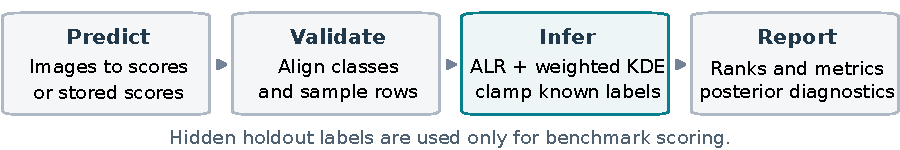
\includegraphics[width=\textwidth]{figures/workflow.pdf}
\caption{End-to-end evaluation: PneumoniaMNIST starts with checkpoint inference; the CivilComments quickstart uses stored scores. Hidden labels enter benchmark scoring only.}
\label{fig:workflow}
\end{figure}

\section{Semi-Supervised Estimator}
Let $p_{imk}$ denote class probabilities, with shape $N\times M\times K$ (binary: $N\times M$). Missing labels use $-1$; each class needs a visible label. Clipped, normalized scores undergo the additive log-ratio transform \citep{aitchison1982} $z_{imk}=\log(p_{imk}/p_{imK})$, yielding $M(K-1)$ features.

With responsibilities $\gamma_{ik}$ and annotation weights $w_i=10$ for visible labels and $1$ otherwise, iterations update Gaussian kernel densities \citep{scott1992}, priors, and posteriors:
\begin{equation}
 f_k(z)=\frac{\sum_i w_i\gamma_{ik}K_h(z-z_i)}{\sum_i w_i\gamma_{ik}},\quad
 \pi_k=\frac{\sum_i w_i\gamma_{ik}}{\sum_i w_i},\quad
 \gamma_{ik}\leftarrow\frac{\pi_k f_k(z_i)}{\sum_c\pi_c f_c(z_i)}.
\end{equation}
Initialization samples from mean model probabilities; visible labels remain clamped. Fixed iterations and explicit bandwidth settings support controlled, reproducible comparisons.

\clearpage
\section{Implementation and Experimental Design}
\paragraph{Reusable interface and reports.}
The prediction adapter aligns class columns; the split utility records sample indices. A scikit-learn-style estimator \citep{pedregosa2011} exports offline HTML, CSV metrics, and JSON statistics. The model-file CLI adds configuration preflight, batched prediction, explicit class order, and input hashes:
\begin{lstlisting}[language=Python]
from ssme_lite import SSMEEstimator
e = SSMEEstimator(max_iter=100, random_state=0)
e.fit(scores, y_partial, model_names=model_names)
e.report(n_draws=100, contribution=True).save("evaluation")
\end{lstlisting}
MIT-licensed version 0.1.0 is \href{https://pypi.org/project/ssme-lite/}{published on PyPI} (\texttt{pip install ssme-lite}); the core needs no PyTorch. Release CI covers Python 3.10--3.14; the current checkout passes 48 tests, also verified from an installed wheel.

\paragraph{Metrics and uncertainty.}
The default report evaluates the estimation pool (visible plus unlabeled samples). Accuracy is the exact posterior expectation of a model's correctness. ROC AUC, average precision (AP), and expected calibration error (ECE) average 100 shared latent-label draws, preserving paired comparisons. AP is the implementation's AUPRC summary; binary ECE uses ten equal-width bins \citep{guo2017}. The interface supports multiclass inputs. Label-sampling intervals describe uncertainty conditional on the fitted posterior.

\begin{table}[!ht]
\centering\small
\renewcommand{\arraystretch}{1.12}
\begin{tabular*}{\textwidth}{@{\extracolsep{\fill}}ccccc@{}}
\toprule
Pipeline & Models & $n_L$ / $n_U$ / $n_H$ & Splits & Bandwidth / epochs\\
\midrule
Checkpoint inference & 7 & 20 / 400 / 204 & 10 & Scott / 100\\
Transfer learning & 5 & 20 / 400 / 204 & 10 & Scott / 100\\
CivilComments quickstart & 7 & 20 / 1,000 / 66,891 & 50 & Reference / 20\\
\bottomrule
\end{tabular*}
\caption{The first two pipelines use PneumoniaMNIST, the main dataset. Counts are visible ($L$), unlabeled ($U$), and held-out ($H$); all runs use weight 10 and 100 label draws.}
\label{tab:protocol}
\end{table}

\paragraph{PneumoniaMNIST: the main end-to-end study.}
The dataset has 4,708 training, 524 validation, and 624 test images \citep{yang2023}. The demo loads seven pretrained checkpoints (one ResNet18, three AutoKeras \citep{jin2023}, three AutoML Vision), runs test-image inference, aligns probabilities, fits SSME, and exports the interactive report. The transfer example freezes an ImageNet ResNet18 \citep{he2016} for 512-dimensional features and trains five sklearn heads on training data only, with fixed hyperparameters. Both pipelines evaluate test data over seeds 0--9; validation is unused for transfer-head selection.

\paragraph{CivilComments: quickstart and reproduction check.}
CivilComments \citep{borkan2019}, used in the SSME paper, supplies seven released score vectors per comment. A half-split protocol collects 50 class-covered runs from seeds 0--58; each class must have a visible label. The reference-code bandwidth rule is the minimum normal-reference ALR bandwidth divided by four. Archived official-code executions establish the reference workflow; this package-level study checks its qualitative gains.

\paragraph{Paired error analysis.}
Split-level error is $e_s=M^{-1}\sum_m|\widehat q_{sm}-q^H_{sm}|$ against held-out truth. Both methods use the same visible labels. Reported reductions $d_s=e_s^L-e_s^{\mathrm{SSME}}$ use descriptive intervals $\bar d\pm t_{.975,S-1}s_d/\sqrt S$; splits, not individual models, are repetitions.

\clearpage
\section{PneumoniaMNIST: Main Results and Diagnostics}
\begin{table}[!ht]
\centering\small
\renewcommand{\arraystretch}{1.08}
\begin{tabular*}{\textwidth}{@{\extracolsep{\fill}}ccccc@{}}
\toprule
 & \multicolumn{2}{c}{MAE (pp)} & \multicolumn{2}{c}{Paired reduction (pp)} \\
\cmidrule(lr){2-3}\cmidrule(lr){4-5}
Metric & Labels only & SSME-Lite & Mean & 95\% CI \\
\midrule
\multicolumn{5}{c}{\textit{Pretrained checkpoints (7 models)}} \\
Accuracy & 5.70 & 2.22 & 3.49 & [2.37, 4.60] \\
AUC & 3.17 & 2.55 & 0.62 & [0.19, 1.04] \\
AP & 2.98 & 2.40 & 0.58 & [-0.06, 1.22] \\
ECE & 3.93 & 2.39 & 1.54 & [0.69, 2.38] \\
\midrule
\multicolumn{5}{c}{\textit{Transfer learning (5 heads)}} \\
Accuracy & 7.11 & 4.16 & 2.95 & [1.00, 4.89] \\
AUC & 4.75 & 3.89 & 0.87 & [-0.59, 2.33] \\
AP & 4.27 & 4.05 & 0.22 & [-1.47, 1.90] \\
ECE & 6.43 & 3.96 & 2.47 & [0.68, 4.26] \\
\bottomrule
\end{tabular*}
\caption{PneumoniaMNIST held-out MAE (pp), ten paired splits. Positive reduction favors SSME-Lite; brackets give unadjusted 95\% $t$ intervals for the paired reduction.}
\label{tab:main}
\end{table}

\paragraph{Accuracy and calibration show the clearest gains.}
Accuracy MAE falls by 61.1\% for pretrained checkpoints and 41.4\% for transfer heads. All twelve models improve in mean Accuracy MAE (Figure~\ref{fig:diagnostics}). Both pipelines also improve ECE, extending the gains to calibration assessment.

\begin{figure}[!ht]
\centering
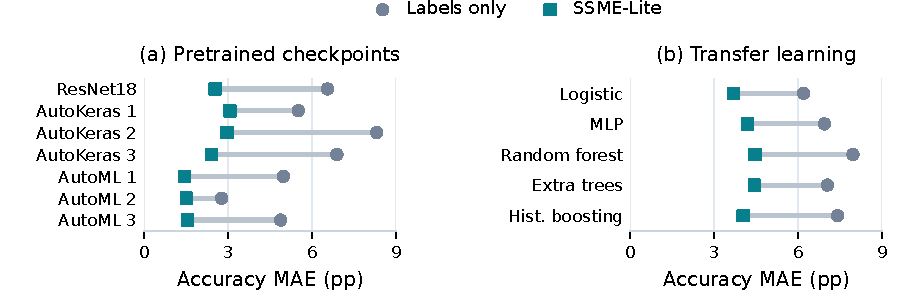
\includegraphics[width=\textwidth]{figures/diagnostics.pdf}
\caption{Accuracy estimation MAE for all seven checkpoints and five transfer heads, averaged over ten held-out splits. Lower is better; every model improves on average.}
\label{fig:diagnostics}
\end{figure}

\paragraph{Improved Accuracy-based model selection.}
Accuracy Top-1 success rises from 23.3\% to 50.0\% for checkpoints and from 25.0\% to 70.0\% for transfer heads. The workflow thus supports both accurate metric estimation and selection of the highest-Accuracy model.

\paragraph{Interpretable model-influence diagnostics.}
For each removed model $m$, sensitivity is
$\mathrm{TV}_m=|U|^{-1}\sum_{i\in U}\frac12\|\gamma_i-\gamma_i^{(-m)}\|_1$.
Removing MLP or logistic regression gives the largest mean TV (0.0465 and 0.0425); the two forest models yield 0.0043 and 0.0030. Initialization, bandwidth, labels, and epochs are fixed. TV quantifies conditional influence under shared full-view initialization.

\clearpage
\section{Extended Evidence and Practical Reuse}
\begin{figure}[!ht]
\centering
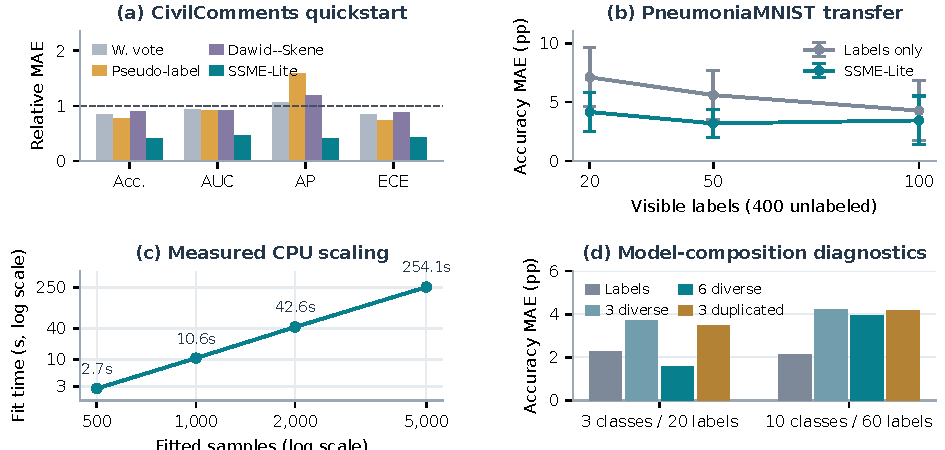
\includegraphics[width=\textwidth]{figures/extensions.pdf}
\caption{Extension study. (a,b) Fixed pool/holdout: 420/204 rows; 30 seeds, nested labels, 95\% $t$ intervals. (c) CPU mean $\pm$ SD over three repetitions, 100 updates. (d) Same three evaluated candidates; ten seeds, fixed 240-row target. MAE units: percentage points.}
\label{fig:extensions}
\end{figure}

\paragraph{Annotation efficiency at a fixed target.}
New seeds 100--129 preserve pool and holdout rows across 20/50/100-label budgets (180 configurations). At 20 labels, checkpoint MAE changes from 5.84 to 3.21 pp and transfer MAE from 7.35 to 4.60 pp: reductions of 45.1\% and 37.3\%. Figure~\ref{fig:extensions}a,b also includes mean-probability estimation. These equal-budget gains use a distinct criterion from cross-budget replacement.

\paragraph{Measured scaling and model composition.}
The 42-condition CPU study measures 500--5,000 rows: fits take 2.73, 10.62, 42.63, and 254.07 s on macOS arm64 with one numerical-library thread. Parallel/batch outputs agree exactly; worker choice is workload-dependent (1,000 rows: 10.62/11.56 s for one/two workers). The 120-condition digits study covers 3/10 classes and diverse/replicated views. Three-class, 20-label MAE is 1.59 pp with six diverse views, versus 3.69 with three and 3.48 with duplicates. Figure~\ref{fig:extensions}d shows two fully class-covered settings.

\paragraph{Original-paper check and delivery.}
CivilComments relative MAEs are 0.41/0.47/0.42/0.42 for Accuracy/AUC/AP/ECE over 50 splits. Baselines include voting, pseudo-labels, and Dawid--Skene \citep{dawid1979}. The checkout adds trusted joblib-to-report configuration and input hashes. Independent auditing checks 342 configurations and 8,478 Accuracy truth values; Appendix~\ref{app:reproduction} links artifacts and commands.

\section{Conclusion}
SSME-Lite unifies prediction, scarce-label evaluation, model selection, and offline reporting. Medical case studies, fixed-target comparisons, and measured execution profiles support its practical reuse.

\clearpage
\begingroup
\raggedright
\hyphenpenalty=10000
\exhyphenpenalty=10000
\setlength{\bibhang}{1.5em}
\setlength{\bibsep}{14pt plus 1pt minus 1pt}
\bibliography{references}
\endgroup
\clearpage
\appendix
\section{Experimental Artifacts and Reproduction}
\label{app:reproduction}

\paragraph{Artifact access.}
OpenI experiment project:\newline
\href{https://openi.pcl.ac.cn/jasonshen/SSME-Lite-2026211240}{openi.pcl.ac.cn/jasonshen/SSME-Lite-2026211240}.
The repository contains the package, paper, frozen predictions, configurations,
raw results, and audit receipts. The base package is also available as
\href{https://pypi.org/project/ssme-lite/0.1.0/}{\texttt{ssme-lite==0.1.0}} on PyPI;
install the accompanying checkout to use the new model-file CLI.

\paragraph{Installation.}
From the repository root, create a clean Python 3.11 environment:
\begin{lstlisting}[basicstyle=\ttfamily\footnotesize]
python -m venv .venv
source .venv/bin/activate
python -m pip install -r reproduction/requirements.txt
python -m pip install --no-deps -e .
\end{lstlisting}
On Windows use \nolinkurl{.venv/Scripts/Activate.ps1}. Fixed-score fits use CPU only.

\paragraph{Main medical experiments.}
Two NPZ files retain all 624 test rows and ordered candidates; SHA256 hashes are
in \nolinkurl{reproduction/inputs/manifest.json}. Run:
\begin{lstlisting}[basicstyle=\ttfamily\footnotesize]
python reproduction/run.py --jobs 2
\end{lstlisting}
The runner refits ten seeds per setting: checkpoints at 20 labels and transfer
heads at 20/50/100 labels, with 400 unlabeled rows, 100 updates, and 100 posterior
draws. At 20 labels it also recomputes model-removal diagnostics. It verifies
splits, model metrics, errors, rankings, and posterior sensitivity against saved
references at absolute tolerance $10^{-10}$. Fresh outputs go to
\nolinkurl{results/reproduction/}. Accuracy MAEs (labels/SSME, pp) are
5.70/2.22 for checkpoints and 7.11/4.16, 5.60/3.19, 4.28/3.45 for transfer.

\paragraph{Model files to an offline report.} Run the included example:
\begin{lstlisting}[basicstyle=\ttfamily\footnotesize]
python examples/model_files.py
ssme-lite check-config results/model_files/config.json
ssme-lite results/model_files/config.json --trust-model-files
\end{lstlisting}
The configuration specifies model paths, evaluation features, partial labels,
ordered classes, and output location. HTML/CSV/JSON outputs include frozen
predictions and input hashes.

\paragraph{Extensions and figure reproduction.} Inspect and rebuild saved evidence:
\begin{lstlisting}[basicstyle=\ttfamily\footnotesize]
python experiments/extensions/audit_results.py
python report/build_report.py
python report/build_extensions.py
\end{lstlisting}
These commands audit saved evidence and regenerate the paper's vector figures.
\nolinkurl{experiments/extensions/README.md} documents fresh pilot/full runs,
30-seed label comparisons, ten-seed composition studies, three-repetition timing,
resume behavior, and the optional 10,000-row server profile. Exact measurement
source snapshots and environments accompany all 342 configurations.

\paragraph{Additional workflows.}
Follow \nolinkurl{docs/reproduction.md} to obtain official CivilComments scores
and run \nolinkurl{experiments/civilcomments/reproduce_official_split.py}; it
collects 50 class-covered splits with 20 labels and 1,000 unlabeled samples.
The same guide provides image-to-report and frozen-ResNet18 training commands.

\end{document}
